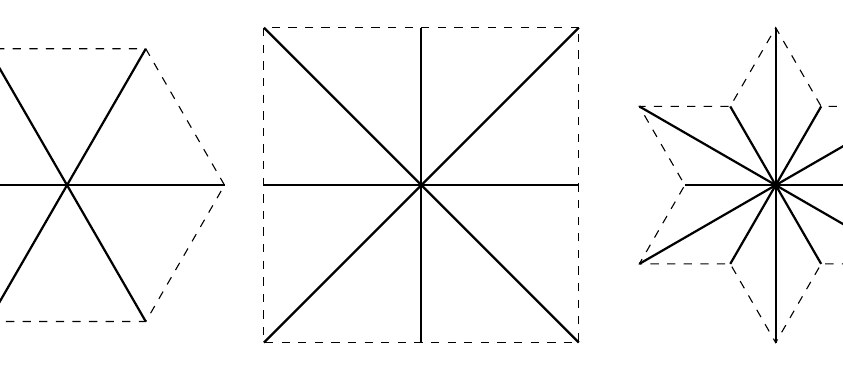
\begin{tikzpicture}
  \def\R{2.0}
  \def\rt3{1.732}
  \def\L{1.732} % R rt3 / 2
  \def\h{1/1.732} % R/( 2 rt3 )

  \useasboundingbox (-5,-2)  rectangle (5,2);

  % Define the coordinates
  \begin{scope}[shift={(-4.5,0)}]
    \coordinate (E) at (\R,0);
    \coordinate (NE) at (0.5*\R,\L);
    \coordinate (NW) at (-0.5*\R,\L);
    \coordinate (W) at (-\R,0);
    \coordinate (SW) at (-0.5*\R,-\L);
    \coordinate (SE) at (0.5*\R,-\L);
    %    -x   x        x = R/rt3
    %  W         E
    %    -x   x
    \draw[dashed] (E) -- (NE) -- (NW) -- (W) --  (SW) -- (SE) -- cycle;
    \draw[thick] (W)  -- (E) ;
    \draw[thick] (SW) -- (NE);
    \draw[thick] (NW) -- (SE);
  \end{scope}

  %\begin{scope}[shift={(0,0)}]
  \coordinate (E) at (\R,0);
  \coordinate (NE) at (\R,\R);
  \coordinate (N) at (0,\R);
  \coordinate (NW) at (-\R,\R);
  \coordinate (W) at (-\R,0);
  \coordinate (SW) at (-\R,-\R);
  \coordinate (S) at (0,-\R);
  \coordinate (SE) at (\R,-\R);

  \draw[dashed] (NE) -- (NW)-- (SW) -- (SE) -- cycle;
  \draw[thick] (W) -- (E);
  \draw[thick] (S) -- (N);
  \draw[thick] (SW) -- (NE);
  \draw[thick] (SE) -- (NW);

  %\end{scope}
  \begin{scope}[shift={(4.5,0)}]
    \coordinate (E) at (\R/\rt3,0);
    \coordinate (NE) at (\L,0.5*\R);
    \coordinate (NE2) at (\h,0.5*\R);
    \coordinate (N) at (0,\R);
    \coordinate (NW) at (-\L,0.5*\R);
    \coordinate (NW2) at (-\h,0.5*\R);
    \coordinate (W) at (-\R/\rt3,0);
    %      N      
    % -z'        z=(R/2,rt3 R/2), 
    %      +                     
    % -z        z' 
    %      S
    \coordinate (SW) at (-\L,-0.5*\R);
    \coordinate (SW2) at (-\h,-0.5*\R);
    \coordinate (S) at (0,-\R);
    \coordinate (SE) at (\L,-0.5*\R);
    \coordinate (SE2) at (\h,-0.5*\R);
    \coordinate (N) at (0,\R);

    \draw[dashed] (E) --  (NE) --  (NE2) -- (N) --  (NW2) --  (NW) -- (W) --  (SW) --  (SW2) -- (S) --  (SE2) --  (SE) -- cycle;

    \draw[thick] (W)  -- (E) ;
    \draw[thick] (SW2) -- (NE2);
    \draw[thick] (NW2) -- (SE2);
    \draw[thick] (S) -- (N);
    \draw[thick] (SW) -- (NE);
    \draw[thick] (NW) -- (SE);
  \end{scope}
\end{tikzpicture}
